\def\offset{2}
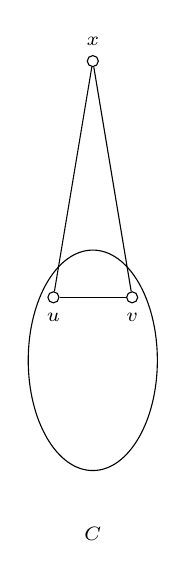
\begin{tikzpicture}

                \tikzstyle{vertex}  = [circle, minimum width=4pt, draw, inner sep=0pt, fill=white]
                \node [vertex, label=above:{\scriptsize$x$},](x) at (2.5, 6) {};
                \node [vertex, label=below:{\scriptsize$u$}](u) at ({0 + \offset}, 3) {};
                \node [vertex, label=below:{\scriptsize$v$}](v) at ({1 + \offset}, 3) {};
                \draw ({0 + \offset + 0.5}, 2.2) ellipse (0.82cm and 1.4cm);
                \node (c) at ({0 + \offset + 0.5}, 0) {\scriptsize$C$};
                \draw (u) -- (v);
                \draw (u) -- (x);
                \draw (v) -- (x);
\end{tikzpicture}

